\section{Pendahuluan}
\subsection{Latar Belakang}
praktikum dilakukan untuk tahu cara melakukan crimmping dengan baik dan benar, serta mengetahui cara routing IPv4 dengan baik dan benar. pengaturan jaringan komputer yang terstruktur dan terencana sangat penting untuk memastikan komunikasi yang efisien dan efektif antara perangkat-perangkat dalam jaringan. Dengan memahami cara melakukan crimping dan routing IPv4, kita dapat membangun jaringan yang handal dan dapat diandalkan.\\
salah satu pembahasan yang penting dalam jaringan komputer adalah pengaturan alamat IP. Alamat IP adalah identifikasi unik untuk setiap perangkat dalam jaringan, dan pengaturan yang tepat sangat penting untuk memastikan komunikasi yang efisien. Routing IPv4 adalah proses pengiriman paket data dari satu jaringan ke jaringan lain berdasarkan alamat IP tujuan. Dengan memahami cara melakukan routing IPv4, kita dapat memastikan bahwa data dikirim dengan benar dan efisien melalui jaringan.\\
beberapa hal penting lainnya seperti subnetting, pengalamatan IP, dan pengaturan routing juga akan dibahas dalam praktikum ini. Subnetting adalah proses membagi jaringan menjadi subnet yang lebih kecil untuk meningkatkan efisiensi dan keamanan. Pengalamatan IP adalah proses memberikan alamat IP yang unik kepada setiap perangkat dalam jaringan. Pengaturan routing adalah proses menentukan jalur terbaik untuk mengirimkan paket data melalui jaringan. Dengan memahami semua aspek ini, kita dapat membangun jaringan komputer yang handal dan efisien.\\
aplikasi praktis dari pemahaman ini sangat luas, mulai dari pengaturan jaringan lokal di rumah hingga pengaturan jaringan besar di perusahaan. Dengan memahami cara melakukan crimping dan routing IPv4, kita dapat membangun jaringan yang handal dan efisien, serta memastikan komunikasi yang efektif antara perangkat-perangkat dalam jaringan.\\

\subsection{Dasar Teori}
%Bagian ini memuat teori-teori dasar yang mendukung pelaksanaan praktikum. Penjelasan mencakup konsep teknis, nama istilah, serta prinsip ilmiah yang relevan. Tujuannya adalah untuk memberikan pemahaman mendalam sebelum praktikum dilakukan.%
1. \textbf{IP Address dan Subnetting}\\
\textbf{IP Address (Internet Protocol Address)} adalah alamat logika yang diberikan ke setiap perangkat dalam jaringan agar dapat saling berkomunikasi. IP address versi IPv4 terdiri dari 32-bit dan biasanya ditulis dalam bentuk desimal bertitik, seperti \textit{\textbf{192.168.0.1}}.\\
\textbf{Subnetting} adalah teknik membagi suatu jaringan IP besar menjadi beberapa jaringan lebih kecil (subnet). Hal ini berguna untuk: Mengelola alamat IP secara efisien, Meningkatkan keamanan jaringan, Mengurangi lalu lintas jaringan, dan Mengorganisir jaringan berdasarkan fungsi atau departemen.\\\\

2. \textbf{CIDR (Classless Inter-Domain Routing)}\\
CIDR adalah metode untuk mengalokasikan dan menulis alamat IP secara fleksibel. CIDR menggunakan \textbf{notasi slash (/)} untuk menunjukkan jumlah bit yang digunakan untuk \textbf{network prefix}, contohnya: \textit{\textbf{/25}} berarti 25 bit untuk network, sisanya 7 bit untuk host, Ini lebih efisien dibanding sistem kelas (class A, B, C) yang lama.\\
CIDR memungkinkan kita membuat subnet yang ukurannya disesuaikan dengan kebutuhan nyata perangkat.\\\\

3. \textbf{Subnet Mask}\\
Subnet mask adalah angka 32-bit yang digunakan untuk memisahkan bagian \textbf{network} dan \textbf{host} dari sebuah IP address.\\
Contoh:\\
\textbf{\textit{255.255.255.0}} $\to$ /24 $\to$ 256 alamat (254 host)\\
\textbf{\textit{255.255.255.128}} $\to$ /25 $\to$ 128 alamat (126 host)\\
Dengan subnetting, kita bisa menghindari pemborosan IP address.\\\\

4. \textbf{Routing}\\
Routing adalah proses pengiriman paket data dari satu jaringan ke jaringan lain. Routing dilakukan oleh perangkat yang disebut \textbf{router}.\\
Jenis-jenis routing:\\
a. staatic routing: routing yang ditentukan secara manual oleh administrator jaringan.\\
b. dynamic routing: routing yang ditentukan secara otomatis oleh perangkat jaringan berdasarkan informasi yang diterima dari perangkat lain.\\
	protokol dari dynamic routing seperti:\\
	1. RIP (Routing Information Protocol): Protokol routing berbasis distance vector yang menggunakan hop count sebagai metrik.\\
	2. OSPF (Open Shortest Path First): Protokol routing berbasis link state yang menggunakan algoritma Dijkstra untuk menentukan jalur terpendek.\\
	3. EIGRP (Enhanced Interior Gateway Routing Protocol): Protokol routing hybrid yang menggabungkan fitur dari distance vector dan link state.\\
5. \textbf{Topologi Jaringan}\\
Topologi jaringan menggambarkan cara perangkat-perangkat dalam jaringan saling terhubung. Dalam kasus ini, digunakan \textbf{topologi star (bintang)} dengan \textbf{router sebagai pusat}, dan setiap departemen memiliki subnet masing-masing yang terhubung ke router.\\\\

6. \textbf{Tabel Routing}\\
Tabel routing adalah daftar berisi jalur-jalur yang diketahui oleh router untuk mencapai jaringan lain. Setiap entri biasanya mencakup:\\
    \textbf{Network Destination}: tujuan subnet.\\
    \textbf{Netmask/Prefix}: ukuran subnet.\\
    \textbf{Gateway}: alamat router yang menjadi penghubung.\\
    \textbf{Interface}: antarmuka fisik/logis yang digunakan.\\
%===========================================================%
\section{Tugas Pendahuluan}
Bagian ini berisi jawaban dari tugas pendahuluan yang telah anda kerjakan, beserta penjelasan dari jawaban tersebut
\begin{enumerate}
	\item pemisalan pertama jika 1 subnet dibagi menjadi 4:\\
	\\untuk departemen R&D 100 perangkat menggunakan CIDR \textbf{\textit{/25}}, dengan IP range \textbf{\textit{192.168.0.0 - 192.168.0.127}}, jumlah Ip(dengan cadangan) 126.\\
	untuk departemen produksi 50 perangkat menggunakan CIDR \textbf{\textit{/26}}, dengan IP range \textbf{\textit{192.168.0.128 - 192.168.0.191}} jumlah Ip(dengan cadangan) 62.\\
	untuk departemen administrasi 20 perangkat menggunakan CIDR \textbf{\textit{/27}}, dengan IP range \textbf{\textit{192.168.0.192 - 192.168.0.223}}, jumlah Ip(dengan cadangan) 30.\\
	untuk departemen marketing 10 perangkat menggunakan CIDR \textbf{\textit{/28}}, dengan IP range \textbf{\textit{192.168.0.224 - 192.168.0.239}}, jumlah Ip(dengan cadangan) 14. \\\\
	pemisalan kedua jika ada 2 subnet dibagi menjadi 2 masing masing 2 subnet:\\
	untuk departemen R&D 100 perangkat menggunakan CIDR \textbf{\textit{0/25}}, dengan IP range \textbf{\textit{192.168.0.0 - 192.168.0.127}}, jumlah Ip(dengan cadangan) 126.\\
	untuk departemen produksi 50 perangkat menggunakan CIDR \textbf{\textit{128/25}}, dengan IP range \textbf{\textit{192.168.0.128 - 192.168.0.256}} jumlah Ip(dengan cadangan) 126.\\
	untuk departemen administrasi 20 perangkat menggunakan CIDR \textbf{\textit{0/25}}, dengan IP range \textbf{\textit{192.168.1.0 - 192.168.1.127}}, jumlah Ip(dengan cadangan) 126.\\
	untuk departemen marketing 10 perangkat menggunakan CIDR \textbf{\textit{128/25}}, dengan IP range \textbf{\textit{192.168.1.128 - 192.168.1.256}}, jumlah Ip(dengan cadangan) 126. \\
	total ada 4 subnet yang ada jaringan diatas.
	\item menggunakan soal 1 dengan pemisalan yang kedua seperti pada gambar dibawah:\\
	\begin{center}
		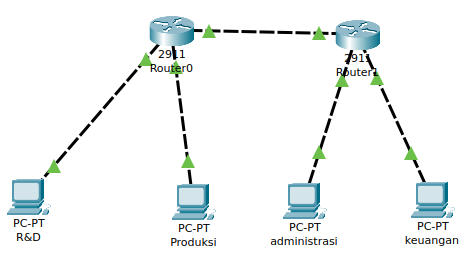
\includegraphics[width=0.8\textwidth]{/home/ichbinwil/kode_kuliah/latex/praktikum-jarkom/Template Laporan Sementara/P1/img/TOPOLOGI.png}
	\end{center}
	
	\item Berikut tabel routing statis internal berdasarkan pembagian subnet:

	\begin{table}[h!]
		\centering
		\begin{tabular}{|l|l|l|l|}
		\hline
		\textbf{Destination Network} & \textbf{Netmask (CIDR)} & \textbf{Gateway} & \textbf{Interface Tujuan} \\ \hline
		192.168.0.0                  & 255.255.255.128 (/25)   & - (direct)       & eth0 (R\&D)               \\ \hline
		192.168.0.128                & 255.255.255.192 (/26)   & - (direct)       & eth1 (Produksi)           \\ \hline
		192.168.0.192                & 255.255.255.224 (/27)   & - (direct)       & eth2 (Administrasi)       \\ \hline
		192.168.0.224                & 255.255.255.240 (/28)   & - (direct)       & eth3 (Keuangan)           \\ \hline
		\end{tabular}
	\end{table}

	\item \textbf{Routing Statis}, karena \textbf{Topologi kecil dan tetap}(anya 4 subnet, tidak sering berubah),
	\textbf{Lebih aman dan hemat sumber daya}dibandingkan dynamic routing,
	\textbf{Konfigurasi mudah dan tidak kompleks} untuk administrator jaringan.
		
\end{enumerate}